%  \documentclass[DIV=12, a4]{scrartcl}
%\documentclass[12pt, a5]{scrartcl}

% \documentclass[a4paper]{report}
% \usepackage[
% % fancytheorems, 
% noindent, 
% %spacingfix, 
% %noheader
% ]{vanilla}


\documentclass[a4paper]{scrreprt}
\usepackage[
fancytheorems, 
noindent, 
% %spacingfix, 
% %noheader,
fancyproofs
]{adam} 

\usepackage{tikz}
\usetikzlibrary{datavisualization}
\usetikzlibrary{datavisualization.formats.functions}

\newcommand{\dd}{\mathrm{d}}

% \usepackage{subfig}

\setcounter{chapter}{-1}

\title{Differential Equations}
% \subtitle{Adam Kelly}
\author{Adam Kelly}
% \date{Michaelmas 2020}
\date{\today}

\begin{document}

\maketitle

\begin{abstract}
	
	% \vspace{2\baselineskip}
	% {\color{red} None of the notes here have been reviewed at all, and are just exactly what was taken down live in the lectures. I would turn around now and come back in a few days, when I have gone back, cleaned things up, fixed explanations and added some structure.}
	% \vspace{5\baselineskip}

	This set of notes is a work-in-progress account of the course `Differential Equations', originally lectured by Dr. John Taylor in Michaelmas 2020 at Cambridge. These notes are not a transcription of the lectures, but they do roughly follow what was lectured (in content and in structure).

	These notes are my own view of what was taught, and should be somewhat of a superset of what was actually taught. I frequently provide different explanations, proofs, examples, and so on in areas where I feel they are helpful. Because of this, this work is likely to contain errors, which you may assume are my own. If you spot any or have any other feedback, I can be contacted at \href{mailto:ak2316@cam.ac.uk}{ak2316@cam.ac.uk}.


	% {\color{red} Notes written upto lecture 6.}
	% During the creation of this document, I consulted a number of other books and resources. All of these are listed in the bibliography. 

\end{abstract}

\tableofcontents

\clearpage

\chapter{Introduction}

Differential equations is a foundational course in applied mathematics, which many courses in the future use as a foundation. This subject studies equations involving \emph{derivatives}, and towards the end, \emph{partial derivatives}. A working knowledge of calculus is essential, but will be briefly reviewed at the start of the course. 


\section{Structure of the Course}

This course is divided into five sections.

\begin{enumerate}
	\item \emph{Basic Calculus}
	
	% This section is a brief review of Calculus, which you should be familiar with.
	% We will treat (informally) derivatives, integrals, Taylor's theorem and the fundamental theorem of calculus. This review will be done through the introduction of $O$ and $o$ notation (for which familiarity is \emph{not} assumed).

	% After this, we take a brief look at functions of several parameters, and the consequential notion of partial derivatives.

	\item \emph{First-Order Linear Differential Equations}
	
	% This section has a different perspective, centering on the questions of \emph{what is a real number} and \emph{what can we assume about them?} This is one of the harder parts of this course, and many of the definitions contain a subtlety that is not present in other sections. 

	\item \emph{Nonlinear First-Order Differential Equations}
	\item \emph{Higher-Order Linear Differential Equations}
	\item \emph{Multivariate Functions and Applications}
	
	% This is a `terminology' section. There is no exciting theorems, mostly notation, definitions, and so on. It is a short section, but it is somewhat boring in that sense.

\end{enumerate}

Everything in the sections above makes up the `course'. If you are wondering what is examinable, it will be everything that was lectured. It is possible that this set of `lecture notes' will contain additional content that was both not in lectures and not examinable. If you want to be sure whether something you are reading here or elsewhere is examinable, you can get a more formal answer in \href{https://www.maths.cam.ac.uk/undergrad/files/schedules.pdf}{the schedules}.

\section{Books}

As with most mathematics courses in Cambridge, you will not need a textbook to follow this course. What is covered in lectures is enough to do both the example sheets and the examinations for this course. Still, you might find that a textbook can provide a different perspective, additional worked examples, and additional material that you may find informative, helpful or fun.

The following books were recommended in the schedules
\begin{itemize}
	\item J. C. Robinson, \emph{An Introduction to Ordinary Differential Equations}.

	\item R. T. Allenby, \emph{Numbers and Proofs}.
	
	This book is readable, easy to understand and clear.

	\item A. G. Hamilton, \emph{Numbers, Sets and Axioms}.
	
	Another readable and clear book, but with a different flavour to the previous book.

	\item H. Davenport, \emph{The Higher Arithmetic}.

	This book can be thought of as showing `where things go next'. It is very interesting, and goes quite a bit beyond this course. It is worth noting however that this book contains no exercises.
\end{itemize}

You should be able to find all of these books in either your college library or the university library.

% \section{Example Sheets}

% As is normal for a 24 lecture course, there will be 4 example sheets. You should be able to have a good go at the first one after lecture 3 or 4.

\section{A Brief Note About These Notes}

This set of notes differs from what was lectured in a number of areas. I have attempted to briefly outline these changes below.

In this set of notes, the review of calculus in the first chapter is done with slightly more rigour than was present in the original lecture course (however, it is still an informal account by any means).


\clearpage


\chapter{Calculus}

To study differential equations, one needs to have a working knowledge of calculus. The goal of this chapter is to review some of the ideas that you (should) have learned previously, but through the introduction of $O$ and $o$ notation. Following this, we will briefly introduce the idea of `functions of several variables', along with partial differentiation.

{\color{red} TODO: This section needs to be rewritten, but my focus for now is on the later (differential equations) part of the course.}

% \section{Differentiation}

% We will begin our review of calculus by defining the notion of the \emph{derivative} of a function. 

% \begin{definition}[Derivative]
% 	Let $f: I \rightarrow \R$ be a function defined on some interval $I \subseteq \R$. The \vocab{derivative} of $f$ 
% 	is the limit
% 	$$
% 	f'(x) = \frac{\dd f}{\dd x} = \lim_{h \to 0} \frac{f(x + h) - f(x)}{h},
% 	$$
% 	provided it exists.
% 	If this limit exists for all $x \in I$, then we say $f$ is \vocab{differentiable} over $I$. 
% \end{definition}

% \begin{example}
% 	The function $f(x) = |x|$ is not differentiable at $x = 0$ as the limit does not exist. 
% \end{example}


% For sufficiently smooth functions (where the derivative exists at each step), we can repeatedly differentiate the function to obtain `higher order derivatives'. These can be defined recursively.

% \begin{definition}[Higher-Order Derivatives]
% 	For a function $f$, we define the \vocab{$n$th derivative of $f$} by
% 	$$
% 	\frac{\dd^n f}{\dd x^n} = \frac{\dd}{\dd x} \left(
% 		\frac{\dd^{n- 1} f}{\dd x^{n-1}}
% 	\right),
% 	$$
% 	with $\frac{\dd^0 f}{\dd x^0} = f$.
% \end{definition}

% It should be noted that we will regularly use three different notations for the derivative of a function $f$: 
% $$
% \frac{\dd f}{\dd x} = f'(x) = \dot{f}(x),
% $$
% which are the Leibniz, Lagrange and Newton notation respectively. Typically we will only use the $\dot{f}(x)$ notation when the independent variable is time.

% \subsection{Rules for Differentiating}

% There are a number of well known properties of derivatives that make them easier to compute.

% \begin{theorem}[Chain Rule]
% 	Let $f(x) = g(h(x))$ for functions $g(x)$ and $h(x)$. Then
% $$
% f'(x) = g'(h(x))\cdot h'(x) = \frac{\dd g}{\dd h} \frac{\dd h}{\dd x}.
% $$
% \end{theorem}

% \begin{theorem}[Product Rule]
% 	Let $f(x) = u(x)v(x)$ for functions $u(x)v(x)$. Then
% 	$$
% 	f'(x) = u'(x) v(x) + u(x)v'(x) = \frac{\dd u}{\dd x} v + u\frac{\dd v}{\dd x}.
% 	$$
% \end{theorem}

% The product rule can be generalized to higher-order derivatives in the following way.\footnote{This should be reminiscent of the Binomial formula, and indeed both can be proved by the same combinatorial argument.}

% \begin{theorem}[Leibniz Rule]
% 	Let $f(x) = u(x)v(x)$ for functions $u(x)$ and $v(x)$. Then
% 	\begin{align*}
% 		f^{(n)}(x) &= \sum_{k = 0}^n \binom{n}{k} u^{(k)} (x) v^{(n - k)}(x)\\
% 		&= u^{(n)}(x) v(x) + n u^{(n)}(x) v'(x) + \cdots + u(x)v^{(n)}(x).
% 	\end{align*}
% \end{theorem}

% \subsection{Orders of Magnitude}

% Before we continue our discussion of differentiation, we will look at two ways of comparing the `size' of functions -- big-$O$ and little-$o$ notation. Before we proceed, it is important to note that these are ways of comparing the \emph{local} behavior of functions. 


% \begin{definition}[Little-$o$ Notation]
% 	We say $f(x) \in o(g(x))$ as $x \rightarrow x_0$ for some $x_0 \in \R\cup \{\infty\}$ if
% 	$$
% 	\lim_{x \to x_0} \frac{f(x)}{g(x)} = 0.
% 	$$
% \end{definition}
% \begin{remark}
% 	Informally, this can be thought of as `$f(x)$ is much smaller than $g(x)$ near $x_0$'. We will often abuse the notation $f(x) = o(g(x))$ to mean $f(x) \in o(g(x))$.
% \end{remark}

% \begin{example}
% 	$x^2 \in o(x)$ as $x \rightarrow 0$, as
% 	$$
% 	\lim_{x \rightarrow 0} \frac{x^2}{x} = \lim_{x \rightarrow 0} x = 0.
% 	$$
% \end{example}

% \begin{definition}[Big-$O$ Notation]
% 	We say that $f(x) \in O(g(x))$ as $x \rightarrow x_0$ for $x_0 \in \R \cup \{\infty\}$ if there exists a positive constant $M$ such that
% 	$$
% 	\lim_{x \to x_0} \left|\frac{f(x)}{g(x)}\right| = M.
% 	$$
% \end{definition}
% \begin{remark}
% 	Informally, this can be thought of as `$f(x)$ can be locally bounded by $g(x)$'
% \end{remark}

% \begin{example}~
% 	    \vspace*{-\baselineskip}
% 	\begin{enumerate}[label=(\roman*)]
% 		\item $x^2 \in O(x)$ as $x \rightarrow 0$
% 		\item $x \not\in O(x^2)$ as $x \rightarrow 0$.
% 		\item $x^2 \in O(x^2)$ for all $x$.
% 		\item $2x^3 + 4x + 12 \in O(x^3)$ as $x \rightarrow \infty$.
% 	\end{enumerate}

% \end{example}

% To see how little-$o$ notation can be used, consider the following proposition.
% \begin{proposition}
% 	For a differentiable function $f(x)$, as $h \rightarrow 0$ we have
% 	$$
% f(x_0 + h) = f(x_0) + f'(x_0)h + o(h).
% 	$$
% \end{proposition}
% \begin{proof}
% 	By the definition of a derivative, as $h \rightarrow 0$ we have
% 	$$
% 	f'(x_0) = \frac{f(x_0 + h) - f(x_0)}{h} + \frac{o(h)}{h}.
% 	$$
% \end{proof}
% This shows that that we can take some nonlinear (but differentiable) function $f$, and approximate it linearly around some point $x_0$.

% \subsection{Taylor's Theorem}

% Imagine you had some smooth function $f$, and you wanted to locally approximate it with a polynomial\footnote{Why would you want to do this? Well polynomials are pretty nice.}. We might start by writing a polynomial
% $$
% p(x) = a_0 + a_1 x + \cdots + a_n x^n,
% $$
% and then we might calculate the derivatives at the point $0$. If o

\chapter{Linear First-Order Differential Equations}

We will now begin the second major part of the course, studying first-order linear differential equations. 
Let's begin by defining some terminiology.

\begin{definition}[ODE]
	A \vocab{ordinary differential equation} or ODE is a differential equation involving functions of variable.
\end{definition}
\begin{definition}[PDE]
	A \vocab{partial differential equation} or PDE is a differential equation which involves functions of more than one variable (and hence will involve partial differential equations).
\end{definition}

\begin{definition}[Order of a DE]
	An \vocab{$n$th order differential equation} is a differential equation where the higehst order derivative in the equation is $n$.
\end{definition}

\begin{definition}
	We say that a differential equation is $\vocab{linear}$ if the dependant variable appears linearly.
\end{definition}

\begin{example}
	The equation $x^2 y + y' = 0$ is a linear first order differential equation.
\end{example}

\section{The Exponential Function}

It turns out that the exponential function is deeply connected to differential equations. Let's consider the following function
$$
f(x) = a^x,
$$
where $a$ is a positive constant.
We are going to differentiate this function from first principles. 
\begin{align*}
	\frac{\dd f}{\dd x} = \lim_{h \to 0} \frac{a^{x + h} - a^x}{h} = a^{x} \lim_{h \to 0} \frac{a^h - 1}{h}.
\end{align*}
What's notable here is that this limit is independent of $x$. Indeed we can just define
$$
\lambda = \lim_{h \to 0} \frac{a^h - 1}{h},
$$
and then we have $\displaystyle \frac{\dd f}{\dd x} = \lambda a^x$.

With this in mind, we are going to define $\exp(x) = e^x$ as the solution to the differential equation
$$
\frac{\dd f}{\dd x} = f(x) \quad \text{with} \quad f(0) = 1.
$$
Therefore `$e$' is the value of $a$ such that 
$$
\lambda = \lim_{h \to 0} \frac{a^h - 1}{h} = 1.
$$

So what is $\lambda$? To answer this, we will need to introduce the \emph{natural logarithm} $\ln x$. We are going to define $\ln x$ to be the inverse of $e^x$, such that
$$
e^{\ln x} = x.
$$
Now let $y(x) = a^{x} = \left(e^{ln a}\right)^x = e^{x \ln a}$. Thus
$$
\frac{\dd y}{\dd x} = (\ln a) e^{x \ln a} =(\ln a) a^x.
$$
Hence $\lambda = \ln a$.

The exponential function plays a central role in differential equations because it is the \emph{
eigenfunction} of the differential operator.

\begin{definition}[Eigenfunction]
The \vocab{eugenfunction} of an operator is unchanged by the action of the operator, except for a multipliciative scaling by some value called the \vocab{eigenvalue}.
\end{definition}

So if we consider 
$$
\frac{\dd}{\dd x} \left(e^{\lambda x}\right) = \lambda e^{\lambda} x,
$$
we have that $e^{\lambda x}$ is the eigenfunction of the operator $\frac{\dd}{\dd x}$, and $\lambda$ is the eigenvalue.


\section{Rules for Linear ODEs}

We are going to look at some rules which will apply for linear ODEs (of any order).

Let's define some terms
\begin{definition}[Homogeneous]
	An ODE is \vocab{homogeneous} if all terms involve the dependant variable or its derivatives (which implies that $y = 0$ is going to be a solution).
\end{definition}

\begin{definition}[Constant Cofficients]
	An ODE has constant coefficients if the independent variable does not appear explicitly in the differential equation.
\end{definition}

\begin{proposition}
	Any linear homogeneous ODE with constant cofficients has solutions of the form $e^{\lambda x}$.
\end{proposition}

\begin{example}
	Consider the differential equation
	$$
5y' - 3y = 0.
	$$
\end{example}
Let's think about this equation. This has to be satisfied for all values of $x$, this implies that the term involving $y'$ and the term involving $y'$ have to have the same \emph{functional dependance}. For example, if we had $y = x^2$ then $y' = 2x$, and then the equation could not be true for all values of $x$. Now we already saw that the exponential function is the eigenfunction of the differential operator, which means that $y$ and $y'$ will have the same functional dependance if the solution is $e^{\lambda} x$, which is why it shows up here.

Because of this, we might try writing
$$
y = Ae^{\lambda x} \implies y' = A \lambda e^{\lambda x},
$$
which would mean that in our differential equation we would have
$$
5A\lambda e^{\lambda x} - 3 A e^{\lambda x} = 0 \implies 5\lambda - 3 = 0.
$$
Then $5 \lambda - 3 = 0$ is the \emph{characteristic equation}, and solving it gives us that $\lambda = \frac{3}{5}$, so $y = Ae^{3x/5}$.

\begin{proposition}
	For linear homogeneous ODEs, any constant multiple of a solution is also a solution.
\end{proposition}

\begin{proposition}
	An $n$th order linear ODE has $n$ independent\footnote{We will discuss later the exact meaning of `independent'.} solutions.
\end{proposition}

For constant coefficient ODEs, this rule follows from the fundamental theorem of algebra, applied to the ODEs characteristic equation (which will be a degree $n$ polynomial). The proof of this theorem in general will be beyond the scope of this course.

Applying this to our equation $5y' - 3y = 0$, we have that $y = Ae^{3x/5}$ is the only solution.

\begin{proposition}
	An $n$th order ODE requires $n$ initial boundary conditions.
\end{proposition}

\section{Inhomogeneous (Forced) First Order ODEs with Constant Coefficients}

An inhomogeneous ODE with constant coefficients is an ODE that has a term that does not involve $y$, but the independet variable $x$ does not appear in the equations. We are going to look at two cases.
\begin{enumerate}
	\item Constant forcing -- where the inhomogeneous term does not depend on $x$
	\item Eigenfunction forcing -- this will be discussed later
\end{enumerate}

Let's begin with an example of constant forcing.
\begin{example}
	The equation
	$$
	5y' - 3y = 10
	$$
\end{example}
This is one type of differential equation which we will solve in a specific way each time.
\begin{proof}[Solution]
	\begin{enumerate}
		\item Write the \emph{general solution} $y = y_p + y_c$, where $y_p$ is the \emph{particular integral} which is one solution to the equation, and $y_c$ is the \emph{complementary function} which is a solution to the corresponding homogeneous equation.
		\item Find $y_p$ by setting $y' = 0$. In this case
		$$
		y = y_p = -\frac{10}{3}.
		$$
		\item Insert the general solution into the differential equation. For our equation,
		$$
		5 y_c ' - 3y_c = 0
		$$
		\item Solve for $y$.
		$$
		y_c = Ae^{3x/5}
		$$
		\item Combine $y_p$ and $y_c$.
		$$
		y = Ae^{3x/5} - \frac{10}{3}.
		$$
	\end{enumerate}
\end{proof}


We will now look at Eigenfunction forcing.
Consider at the following example problem. 

\begin{example}
	In a sample of rock, isotope A decays into isotope $\mathrm{B}$ at a rate proportional to $a$, the number of nuclei of $\mathrm{A},$ while $\mathrm{B}$ decays into isotope $\mathrm{C}$ at a rate proportional to $b,$ the number of nuclei of $\mathrm{B}$. Find $b(t)$.
\end{example}
\begin{proof}[Solution]
	Let's say that $A$ decays into $B$ at a rate of $k_a a$, and $B$ decays into $C$ at a rate of $k_b b$.
	We can then form the following differential equations.
	\begin{align*}
		\frac{\dd a}{\dd t} &= -k_a a \implies a = a_0 e^{-k_a t} \\
		\frac{\dd b}{\dd t} &= k_a a - k_b b,
	\end{align*}
	that is
	$$
	\dot{b} + k_b b = k_a a = k_a a_0 e^{-k_a t}.
	$$
	We call the rightmost term the \emph{forcing term}, and it is an eigenfunction of the differential operator.

	We will procede as before and write down the particular integral. We might guess that $b_p = ce^{-k_a t}$, and then we can plug that into our previous equation to get
	$$
	-k_a c + k_b c = k_a a_0 \implies c = \frac{k_a a_0}{k_b - k_a}.
	$$
	Then the general solution is $b = b_p + b_c$, so we plug this into the equation and we get $\dot{b}_c + k_b b = 0$, and $b_c = De^{-kt}$, and hence
	$$
b = \frac{k_a}{k_b - k_a} a_0 e^{-k_a t} + D e^{-k_b t}.
	$$

	Now we deal with initial conditions. At $t = 0$, we have $b = 0$. This implies that $D = -c$, and hence $$b = \frac{k_a}{k_b - k_a} a_0 \left(e^{-k_a t} - e^{-k_b t}\right)$$
	We can try and sketch what this will look like as a function of time
	\begin{center}
		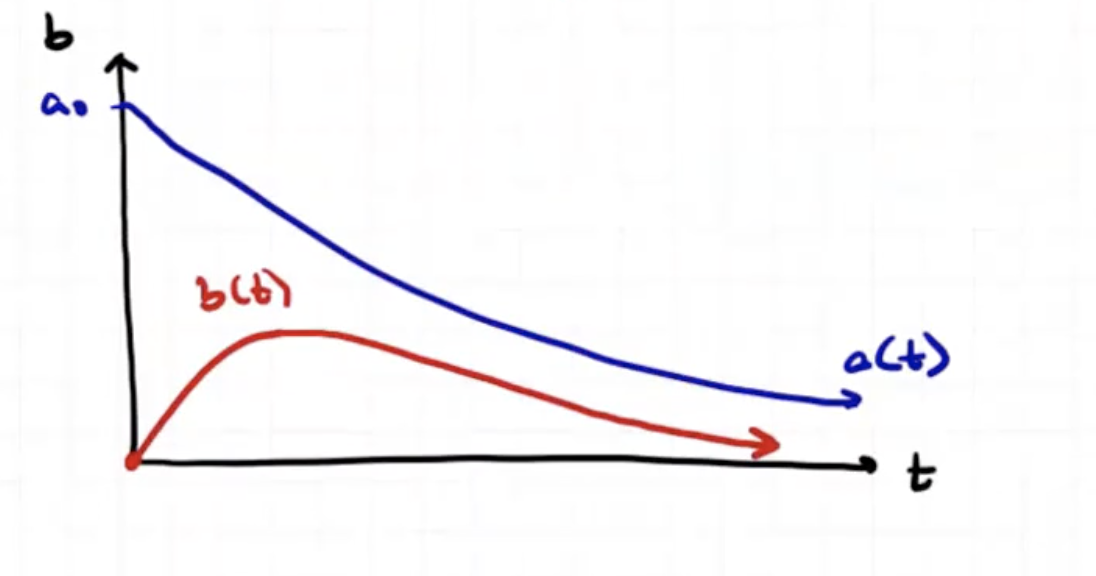
\includegraphics[width=0.6\textwidth]{eigenfunction-forcing.png}
	\end{center}
	Dividing,
	$$
	\frac{b(t)}{a(t)} = \frac{k_a}{k_b - k_a} \left[1 - e^{(k_a - k_b)t}\right].
	$$
	This result allows us to determine the dating of rocks by the proportion of isotopes.
\end{proof}

\section{First-Order ODEs with Non-Constant Coefficients}

Here, we will consider equations of the form
$$
a(x)y' + b(x)y = c(x).
$$
We may also write this in \emph{standard form}
$$
y' + p(x)y = f(x).
$$

We can solve this using the technique of \vocab{integrating factors}.

Consider the standard form, and multiply by $\mu$.
Then we have
$$
\mu y' + (\mu p) y = \mu f = (\mu y)',
$$
if $\mu p = \mu'$, by the product rule.


Hence, we want $p = \frac{\mu'}{\mu}$, so we have
$$
\int p \dd x = \int \frac{\mu '}{\mu} \dd x = \ln \mu
$$
Exponentiating both sides, we have
$$
\mu = e^{\int p(x) \dd x}.
$$

Then our equation becomes
$$
(\mu y)' = f(x) \mu \implies \mu y = \int \mu f,
$$
so we just need to integrate and solve for $y$.

\section{Discrete Equations}

We will now move on to discuss Discrete equations.

\begin{definition}[Discrete Equations]
A \vocab{discrete equation} is an equation involving a function that is evaluated at a discrete set of points.	
\end{definition}

\subsection{Numerical Integration}

We are going to consider the process of solving a differential equation on a computer.
Consider a discrete representation of some function $y(x)$.

\begin{center}
	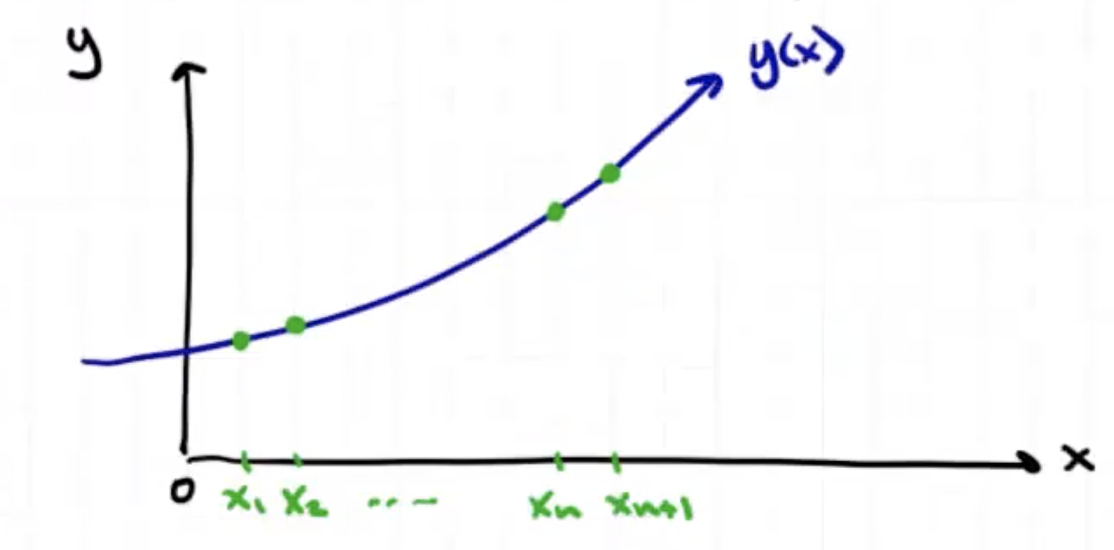
\includegraphics[width=0.6\textwidth]{discrete.png}
\end{center}

We are going to want to approximate the derivative of this function.
One approximation to $\dd y / \dd x$ is
$$
\left.\frac{\dd y}{\dd x}\right|_{x_n} \approx \frac{y_{n + 1} - y_{n}}{h}. 
$$
This is known as \vocab{forward-Euler}, and it is not the best representation!

\begin{example}
	Consider the equation
	$$
	5y' - 3y = 0.
	$$
	We can translate this using the forward-Euler approximation to a discrete equation
	$$
5 \frac{y_{n + 1} - y_n}{h} - 3y_n = 0,
	$$
	that is
	$$
y_{n + 1} = \left(1 + \frac{3h}{5}\right)y_n
	$$
	This is a `recurrence relation'. We can apply this continually, so that we have
	$$
	y_n = (1 + 3h/5)y_{n - 1} = \cdots = (1 + 3h/5)^n y_0.
	$$
\end{example}

We can write this as
$$
y_n = \left(1 + \frac{3xn}{5n}\right)^n y_0,
$$
and Euler defined the exponential function as
$$
\exp(x) \equiv \lim_{n \to \infty} \left(1 + \frac{x}{n}\right)^n,
$$
so 
$$
\lim_{n \to \infty} y_n = y_0 e^{3x/5},
$$
as we would expect.

For a finite $n$, it's notable that $y_n < y(x)$

\subsection{Series Solutions}

Now we are going to introduce a powerful way to solve ODEs, by seeking solutions in the form of an infinite power series. We are going to try to find solutions of the form
$$
y(x) = \sum_{n = 0}^{\infty} a_n x^n,
$$
which will involve plugging this form into the DE to find the coefficients.

Let's return to our original example,
$$
5y' - 3y = 0.
$$

\begin{example}[Series Solutions]
	We will solve the equation $5y' - 3y = 0$.
	Let $y(x) = \sum_{n = 0}^{\infty} a_n x^n$, and $y' = \sum_{n = 0}^{\infty} n a_n x^{n - 1}$.
	Multiplying the original equation by $x$, we have
	$$
	xy' = \sum_{n = 0}^{\infty} n a_n x^{n} = \sum_{n = 1}^{\infty} n a+n x^n,
	$$
	and
	$$
	xy =  \sum_{n = 0}^{\infty} a_n x^{n + 1} = \sum_{m = 1}^{\infty} a_{m - 1} x^m.
	$$
	Plugging these back into the equation,
	$$
5	\sum_{n = 1}^{\infty} n a_n x^n - 3 \sum_{n = 1}^{\infty} a_{n - 1}x^n = 0,
	$$
	or 
	$$
	\sum_{n = 1}^{\infty} x^n (5n a_n - 3a_{n - 1}) = 0.
	$$
	The key observation here is that this must hold for all $x$. This can only happen when
	$$
	5n a_n - 3 a_{n - 1} = 0 \implies a_n = \frac{3}{5n} a_{n - 1}.
	$$
	We will solve this by iterating, so we get
	$$
	a_n = \left(\frac{3}{5}\right)^n \frac{a_0}{n!},
	$$
	hence $y = a_0\left(1 + \frac{3}{5}x + \frac{(3x/5)^2}{2!} + \cdots\right)$,
	which is the power series expansion for $e^{3x/5}$.
	Hence we can conclude
	$$
y = a_0 e^{3x/5}.
	$$
\end{example}

\chapter{Nonlinear First-Order Differential Equations}

Before, we considered only equations where the differential equations were linear. We will now consider equations of the form
$$
Q(x, y) \frac{\dd y}{\dd x} + P(x, y) = 0,
$$
for some functions $P$ and $Q$.

In general, these equations will be very hard to solve. It is quite easy to write down an equation that doesn't have a solution. We will consider two special cases where we can infact solve the equation.

The first method of solving differential equations is \emph{seperation of variables}, which will work for seperable equations.

\begin{definition}
A differential equation is separable if it can be written in the form
$$
q(y) \dd y = p(x) \dd x.
$$
We can solve for $y(x)$ by integrating both sides.
\end{definition}

The other type is an \emph{exact equation}.

\begin{definition}
	A differential equation is an exact equation if and only if 
	$$
	Q(x, y) \dd y + P(x, y) \dd x 
	$$
	is an \vocab{exact differential} of a function $f(x, y)$.
\end{definition}

By an exact differential, we mean $\dd f = Q \dd y + P \dd x$.

If this holds, then this implies that $\dd f = 0$, and the solution can be found by integrating.
To check that this exists (and to find $f(x, y)$), we will use the multivariate chain rule:
$$
\dd f=\frac{\partial f}{\partial x} \dd x+\frac{\partial f}{\partial y} \dd y
$$
so
$$
\dd f = 0 \implies \frac{\partial f}{\partial x} + \frac{\partial f}{\partial y} \frac{\dd y}{\dd x} = 0.
$$
Let's go back and compare this with the general form of our differential equation. From this, if out general form is an exact differential, then there exists $f(x, y)$ such that $P(x, y) = \frac{\partial f}{\partial x}$, and $\frac{\partial f}{\partial y} = Q(x, y)$.

What we want to do this is turn this into a relation between $P$ and $Q$, so that we can test if our equation is an ODE. We get
$$
\frac{\partial^2 f}{\partial y \partial x} = \frac{\partial P}{\partial y} \quad \text{and} \quad \frac{\partial^2 f}{\partial x \partial y} = \frac{\partial Q}{\partial x}.
$$
So
$$
\frac{\partial P}{\partial y} = \frac{\partial Q}{\partial x}.
$$
This is a useful equation to show that an ODE is exact. If this equation holds throughout a \emph{simply connected} domain $D$, then $P \dd x + Q \dd y$ is an exact differential of a single valued function $f(x, y)$ in $D$.

To explain what simply connected is, in 2D, a simply connected domain is a domain that has no holes, for example 
\begin{center}
	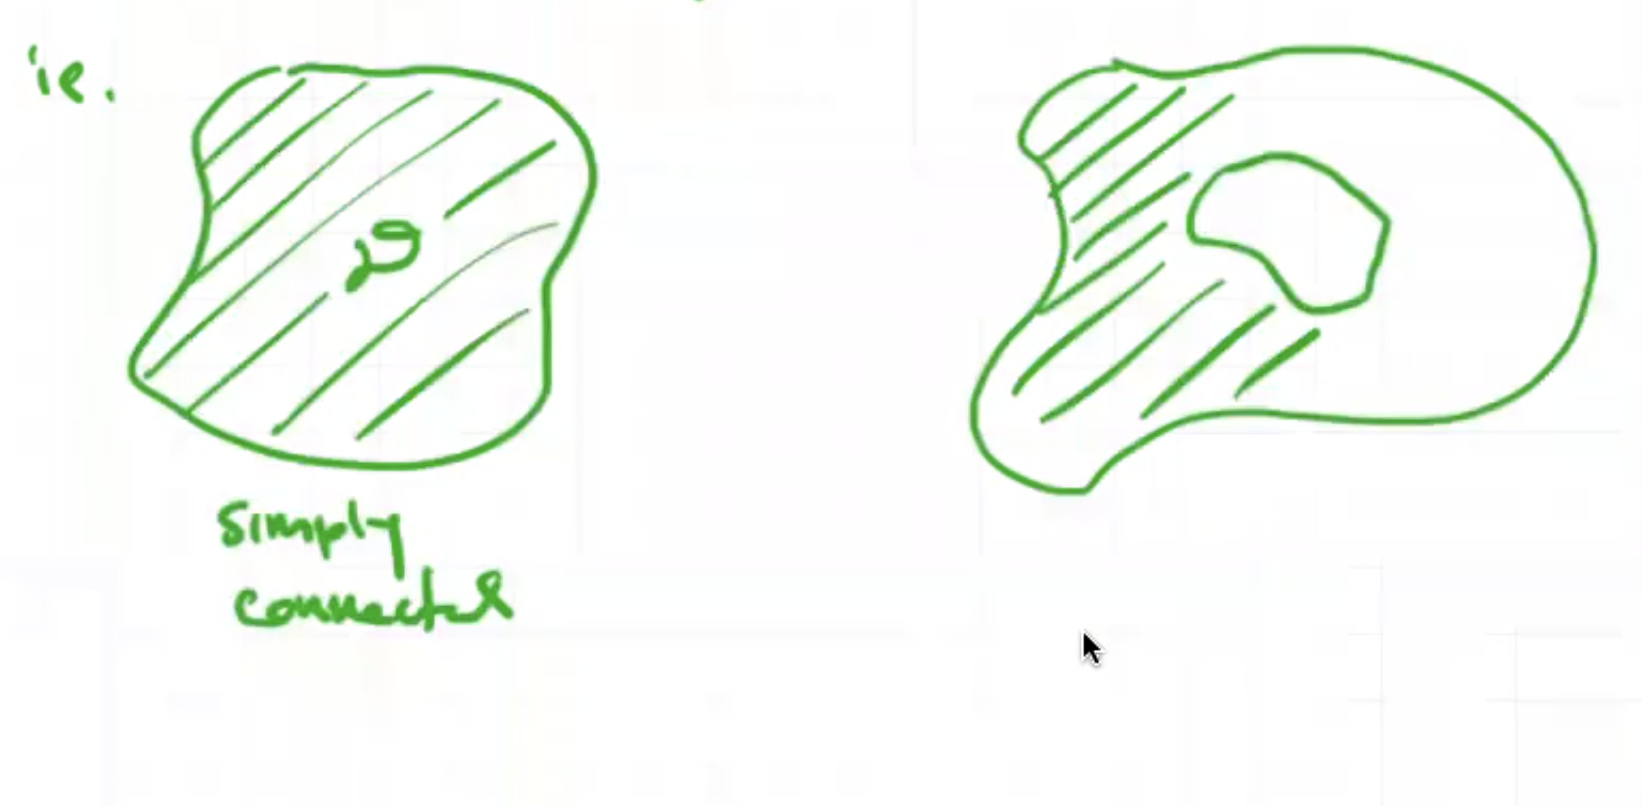
\includegraphics[width=0.6\textwidth]{simply-connected.png}
\end{center}

If the condition, holds then we can try and find $f(x, y)$. We will do this by integrating.

\begin{example}
	Consider the following differential equation
	$$
	6y(y - x)\frac{\dd y}{\dd x} + (2x - 3y^2) = 0
	$$
	Here we have
	$$
	P = 2x - 3y^2, \quad Q = 6y(y - x).
	$$
	Then as
	$$
	\frac{\partial P}{\partial y} = \frac{\partial Q}{\partial x} = -6y,
	$$
	this is an exact equation.

	So we have
	$$
	\left.\frac{f}{x}\right|_{u} = P = 2x - 3y^2,
	$$
	and we can integrate with respect to $x$ to get
	$$
f= x^2 - 3xy^2 + h(y),
	$$
	where $h$ is some function only of $y$.
	We also have
	$$
	\left.\frac{\partial f}{\partial y}\right|_x = -6xy + \frac{\dd h}{\dd y} = 6y(y - x),
	$$
	hence
	$$
	\frac{\dd h}{\dd y} = 6y^2 \implies h = 2y^3 + C,
	$$
	and thus
	$$
	f(x, y) = x^2 - 3xy^2 + 2y^3 + C,
	$$
	which is the general solution to our differential equation.
\end{example}
% \end{aside}


\end{document}
